%%%%%%%%%%%%
%
% $Autor: Wings $
% $Datum: 2019-03-05 08:03:15Z $
% $Pfad: Programming.tex $
% $Version: 4250 $
% !TeX spellcheck = en_GB/de_DE
% !TeX encoding = utf8
% !TeX root = filename 
% !TeX TXS-program:bibliography = txs:///biber
%
%%%%%%%%%%%%


\chapter{Visual Studio Code}

The ac{sw} tool to be used as editor in the project development is one of the key aspects to consider, in order to set the project's background in place. There are plenty of options to consider for this matter, however taking into account the projects capabilities and constraints, there was one clear option for the implementation. \ac{vscode} is a free editor from Microsoft, which has the enormous advantage of having a plug-in specialized for all products of the manufacturer Espressif \cite{Espressif:2022}, to be programmed and flashed.

In this section, will be presented the different stages of the implementation, from basic installation, to basic initial test on the \ac{sw} and \ac{hw} communication.

%%%%%%%%%%%%%%%%%%%%%%%%%%%%%%%

\section{Installation and setup}

The first thing to make sure is that everything needed to start the project with \ac{vscode} is properly installed and ready to go. Next it is going to be presented and overview to go over the entire setup process, and explain every step to get things working properly.

Even if \ac{vscode} is already installed on the machine, to give quick glance over this section is crucial, in order to make sure that the same direction is being followed before starting the project. 

Obvious to mention, but also it is clear set that if it is the first time installing \ac{vscode}, it is highly recommend completing all of the steps in this section. With no more to add. Let’s jump in!

\begin{enumerate}
    \item Download the executable file.
    \begin{itemize}
        \item You may access the file from the link bellow.
        \begin{description}
            \item[Download Link:] \url{https://code.visualstudio.com/download}
        \end{description}
    \end{itemize}
    \item Click the option Download.
    \begin{itemize}
        \item Select the option that fits the operating system of the machine where \ac{vscode} will be installed. (e.g. Windows) 
        \item \ac{vscode} version 1.73 will be used among this report.
    \end{itemize}
    \begin{figure}  [H]
        \begin{center}
            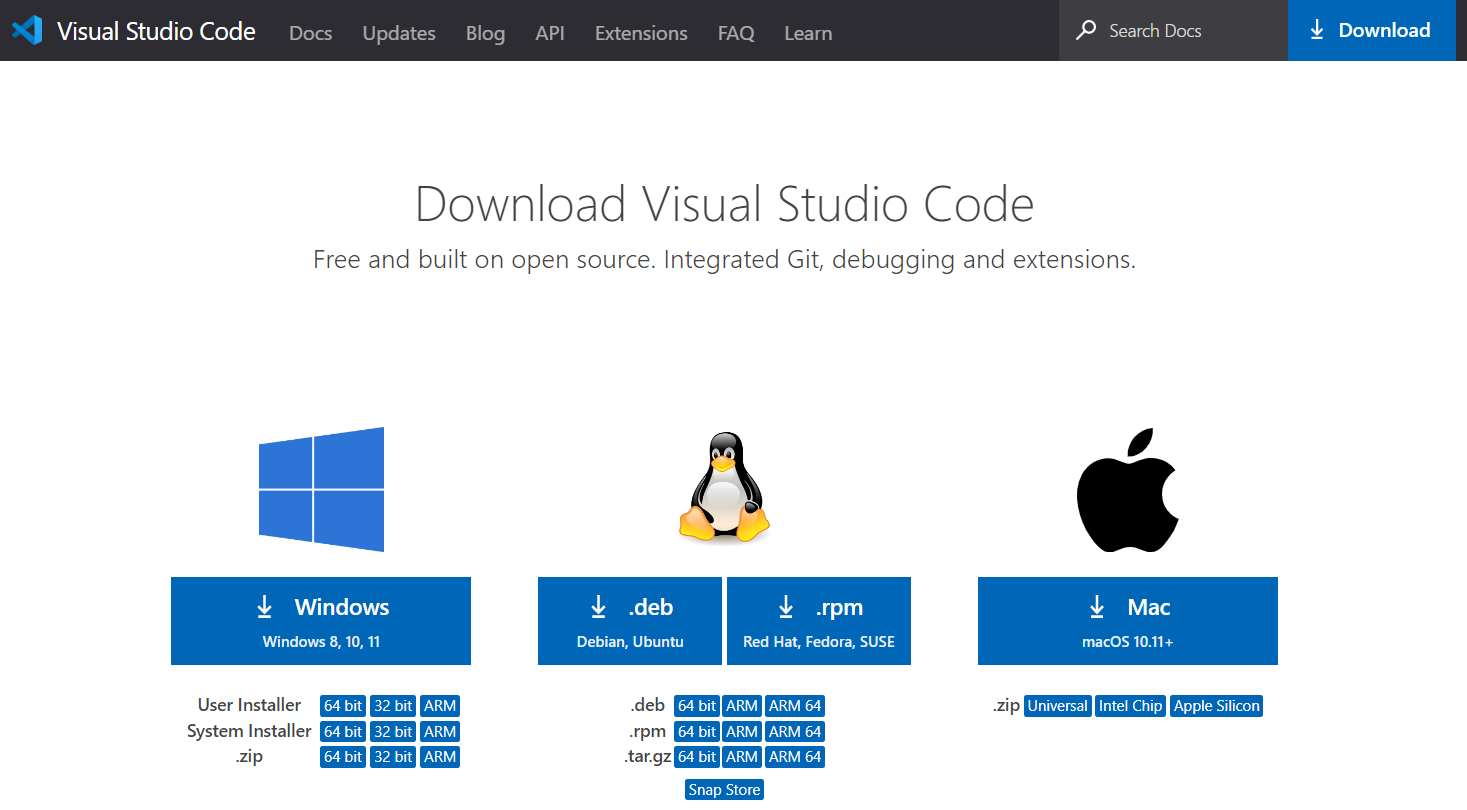
\includegraphics[width=12cm]{ESP32/VSCodeDownload}
            \caption{Visual Studio Code Download Options.} 
            \label{fig:Visual Studio Code Download Options.}
            \footnotesize \textbf{Reference:} \cite{Microsoft:2022}
        \end{center}
    \end{figure}
    \item Double click the downloaded file.
    \begin{itemize}
        \item File is stored under the name: VSCodeUserSetup-x64-1.73.0.exe
        \item Now a dialogue box appears.
        \item Select "I accept the agreement".
        \item Select "Next >".
    \end{itemize}
    \begin{figure}  [H]
        \begin{center}
            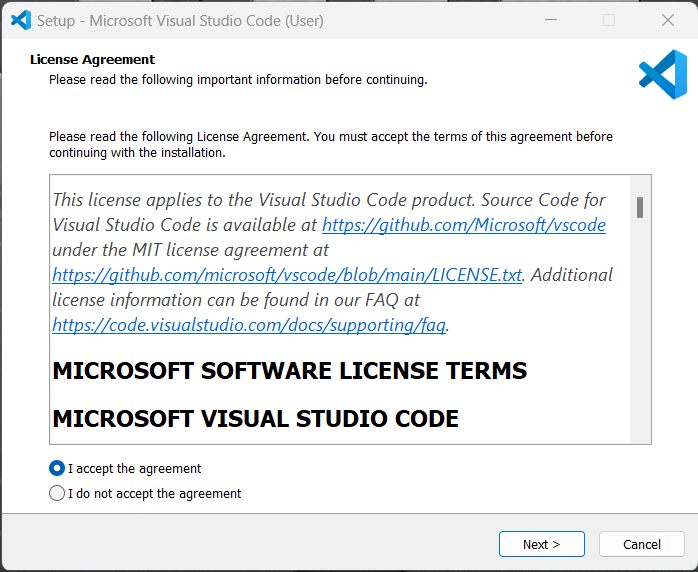
\includegraphics[width=10cm]{ESP32/VSCodeInst1}
            \caption{Visual Studio Code License Agreements.} 
            \label{fig:Visual Studio Code License Agreements.}
        \end{center}
    \end{figure}
    \item Select a folder by clicking Browse or just follow the default path.
    \begin{itemize}
        \item Please note that 348.3 MB are required to be free on your device to complete the installation.
        \item Select "Next >".
    \end{itemize}
    \begin{description}
        \item[Rrecommendation: ] Leave Default path.
    \end{description}
    \begin{figure}  [H]
        \begin{center}
            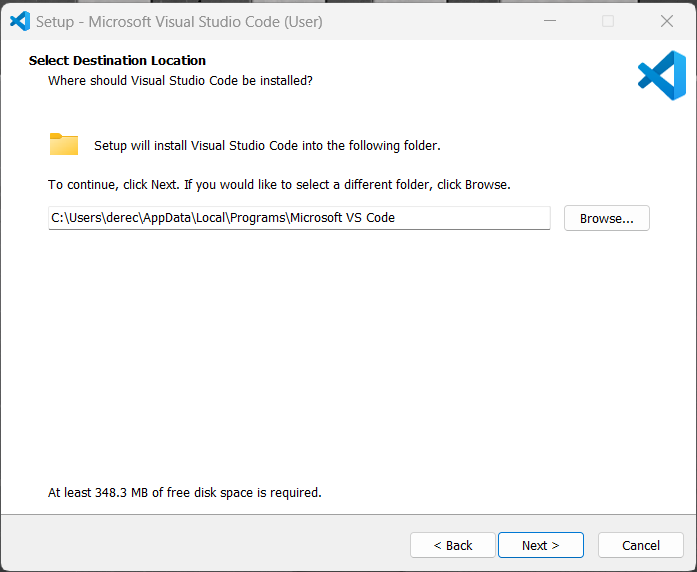
\includegraphics[width=10cm]{ESP32/VSCodeInst2}
            \caption{Visual Studio Code Destination Location.} 
            \label{fig:Visual Studio Code Destination Location.}
        \end{center}
    \end{figure}
    \item Select the Start Menu Folder.
    \begin{description}
        \item[Rrecommendation: ] Leave Default path.
    \end{description}
    \begin{figure}  [H]
        \begin{center}
            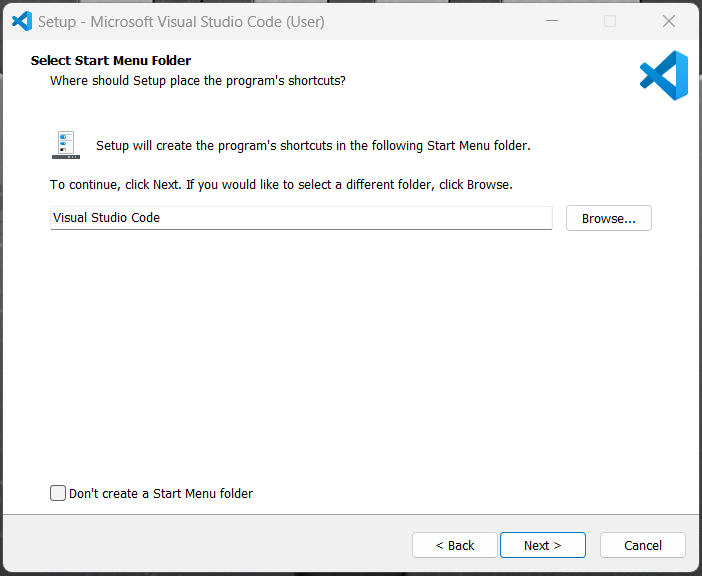
\includegraphics[width=10cm]{ESP32/VSCodeInst3}
            \caption{Visual Studio Code Start Menu Folder.} 
            \label{fig:Visual Studio Code Start Menu Folder.}
        \end{center}
    \end{figure}
    \item Select Additional Tasks.
    \begin{description}
        \item[Rrecommendation: ] Leave Default path.
    \end{description}
    \begin{figure}  [H]
        \begin{center}
            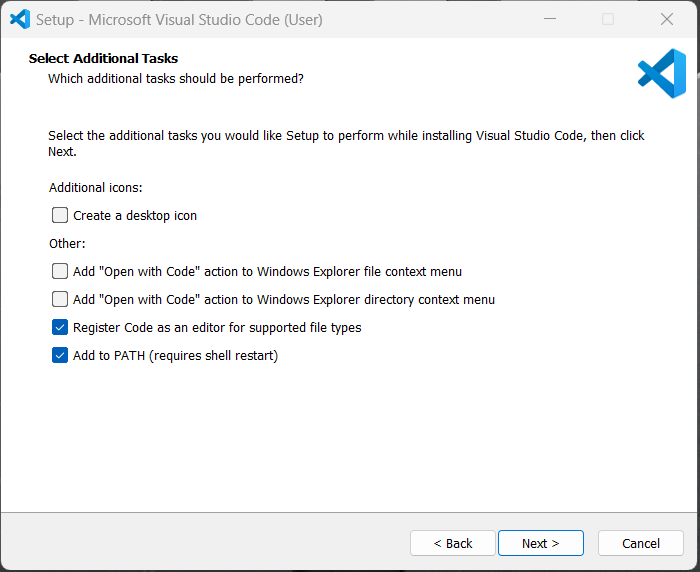
\includegraphics[width=10cm]{ESP32/VSCodeInst4}
            \caption{Visual Studio Code Additional Tasks.} 
            \label{fig:Visual Studio Code Additional Tasks.}
        \end{center}
    \end{figure}
    \item Select Install.
    \begin{figure}  [H]
        \begin{center}
            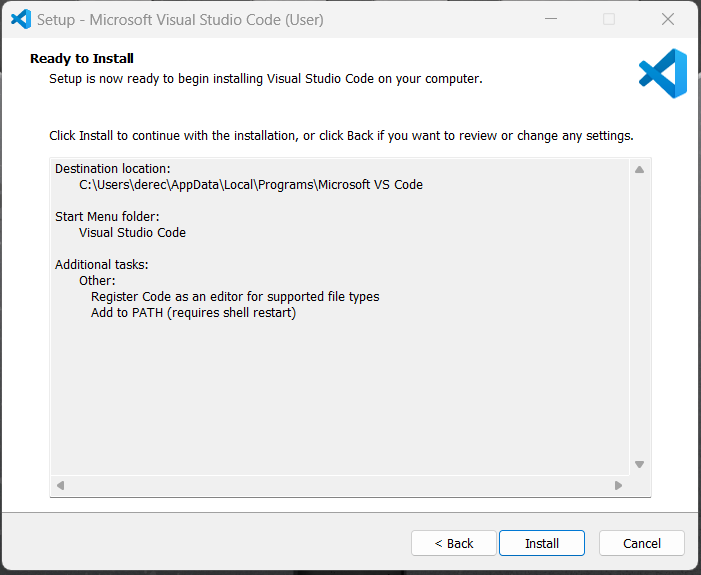
\includegraphics[width=10cm]{ESP32/VSCodeInst5}
            \caption{Visual Studio Code Install.} 
            \label{fig:Visual Studio Code Install.}
        \end{center}
    \end{figure}
    \item Click Finish to exit Setup. Check in the check box to launch \ac{vscode} right now.
    \begin{figure}  [H]
        \begin{center}
            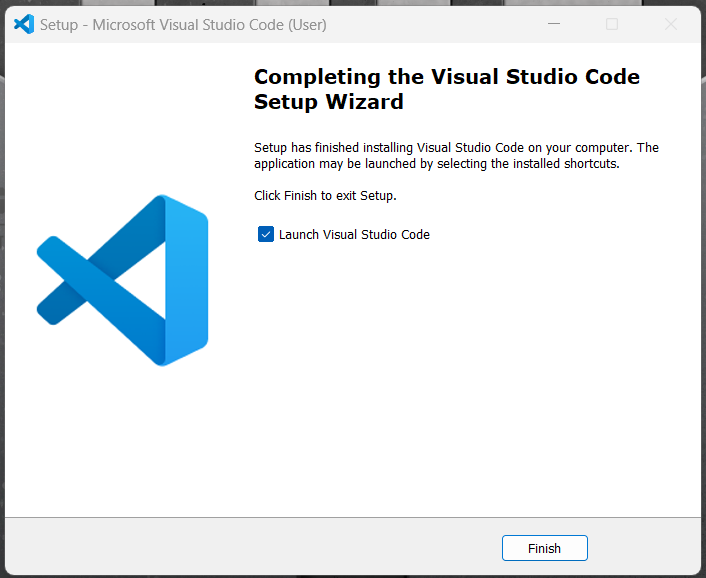
\includegraphics[width=10cm]{ESP32/VSCodeInst6}
            \caption{Visual Studio Code Finished Installation.} 
            \label{fig:Visual Studio Code Finished Installation.}
        \end{center}
    \end{figure}
    \item Open Visual Studio Code and select ``New File'' to create a new file as a test.
    \begin{figure}  [H]
        \begin{center}
            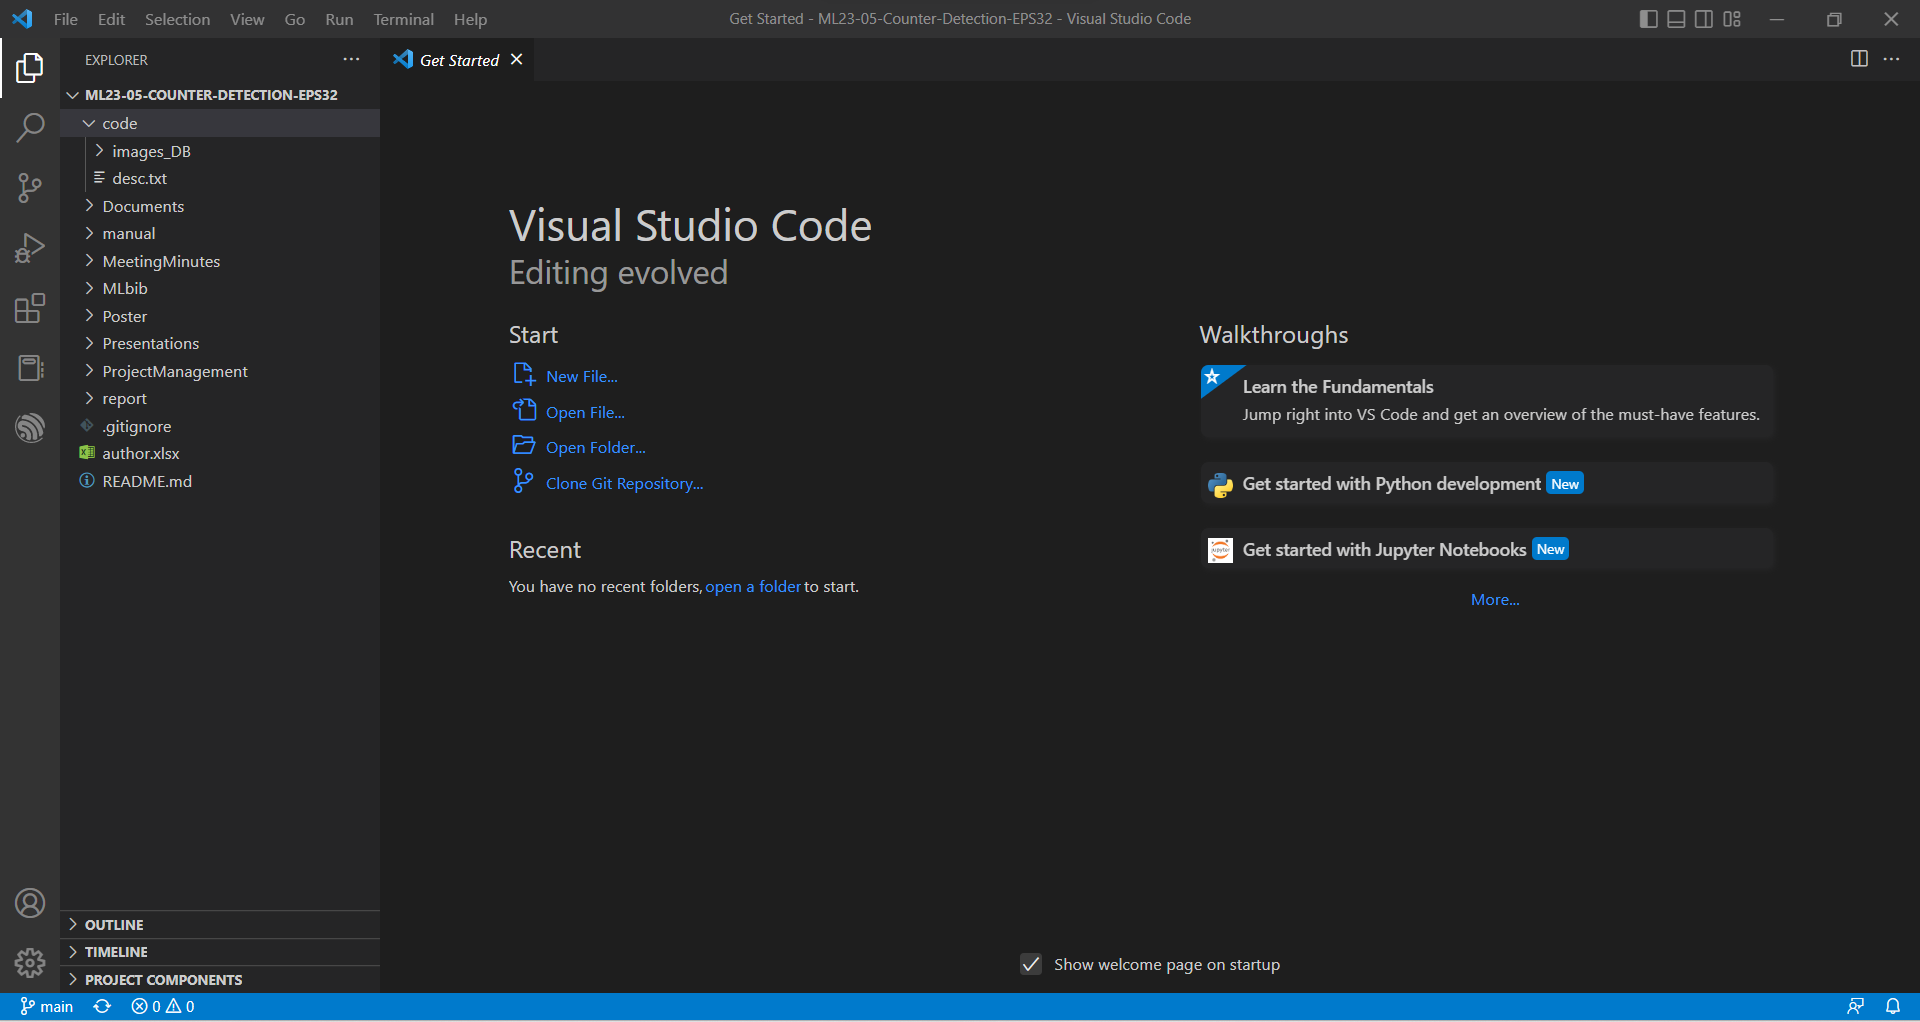
\includegraphics[width=12cm]{ESP32/VSCodeInst7}
            \caption{Visual Studio Code Initial Window.} 
            \label{fig:Visual Studio Code Initial Window.}
        \end{center}
    \end{figure}
    \item For this test, select Python as development environment. 
    \begin{itemize}
        \item In the new window write a basic Hello World, print function
        \item Use this code line: print("Hello ESP32! :)")
    \end{itemize}
    \begin{figure}  [H]
        \begin{center}
            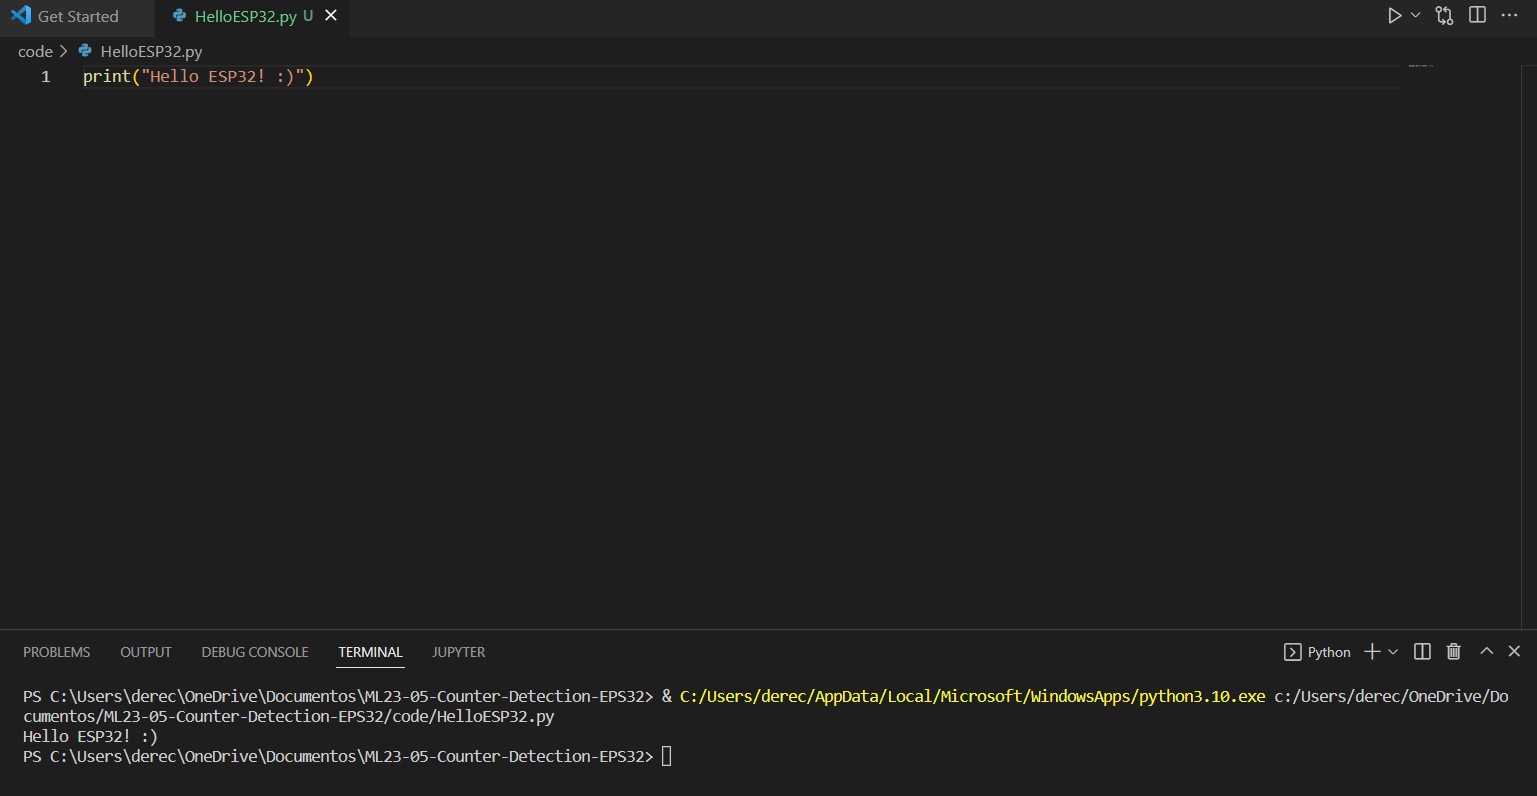
\includegraphics[width=12cm]{ESP32/VSCodeInst8}
            \caption{Visual Studio Code ``Hello ESP32 Basic Code''.} 
            \label{fig:Visual Studio Code "Hello ESP32 Basic Code."}
        \end{center}
    \end{figure}
\end{enumerate}

Congratulations. \ac{vscode} is properly installed and ready to use.

%%%%%%%%%%%%%%%%%%%%%%%%%%%%%%%
\section{ESP-IDF Plug-in}

ESP-IDF is the official development framework for the ESP32 family chips, in \ac{vscode}. This tool is recommended over some other options, such as Arduino IDE, because of the capability to offer more powerful applications. With this versatile plug-in it is possible to develop, build, flash, monitor and debug the code loaded in to ESP32 Devices. For this development is recommended to use version v4.4.3 (latest available), next it will be presented the setup process to get everything ready.

\begin{enumerate}
    \item Open \ac{vscode}.
    \item Open the Extensions view.
    \item Search the extension: "esp-idf"
    \item Select Install option on v1.5.1.
    \begin{figure}  [H]
        \begin{center}
            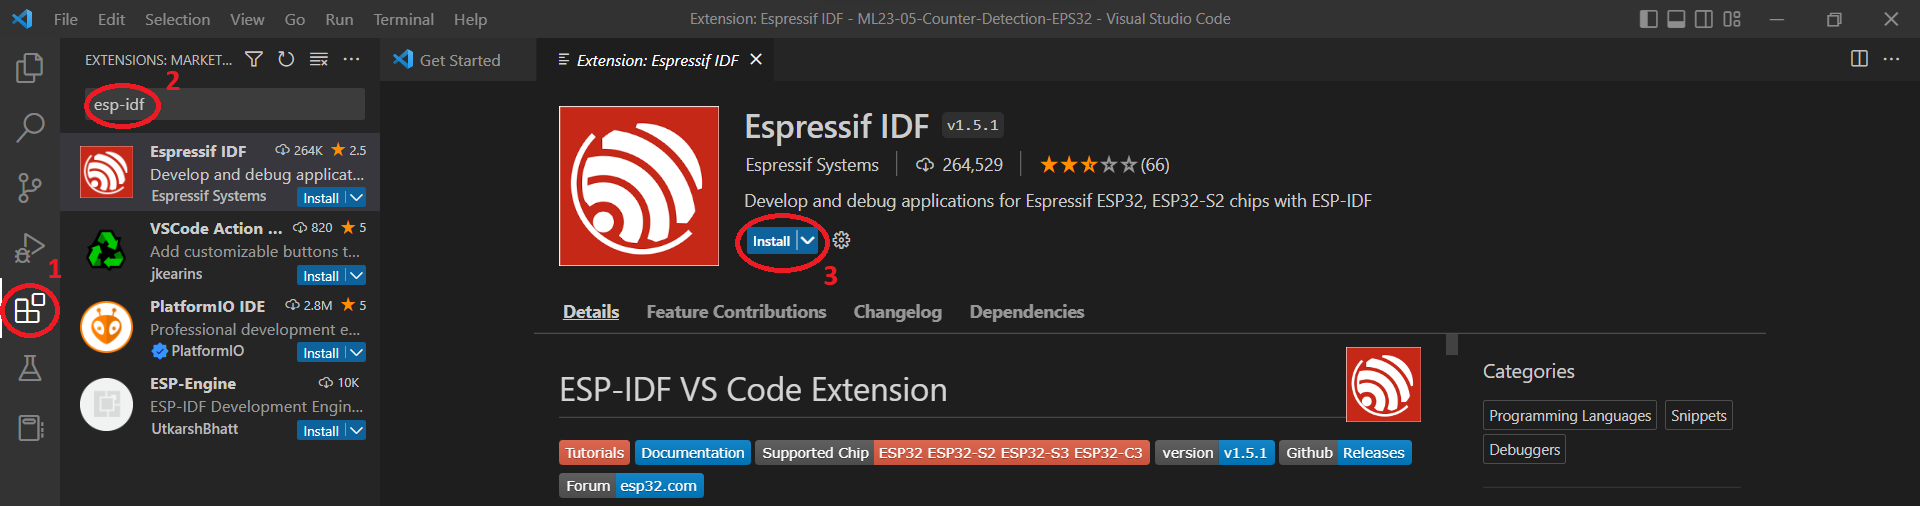
\includegraphics[width=12cm]{ESP32/ESPIDFInst1}
            \caption{Visual Studio Code Install Extension "esp-df".} 
            \label{fig:Visual Studio Code Install Extension "esp-df".}
        \end{center}
    \end{figure}
    \item Select the ESP-IDF: Configure ESP-IDF extension option.
    \item Choose "Express", as the best suited option for the project.
    \item Select Install option.
    \begin{figure}  [H]
        \begin{center}
            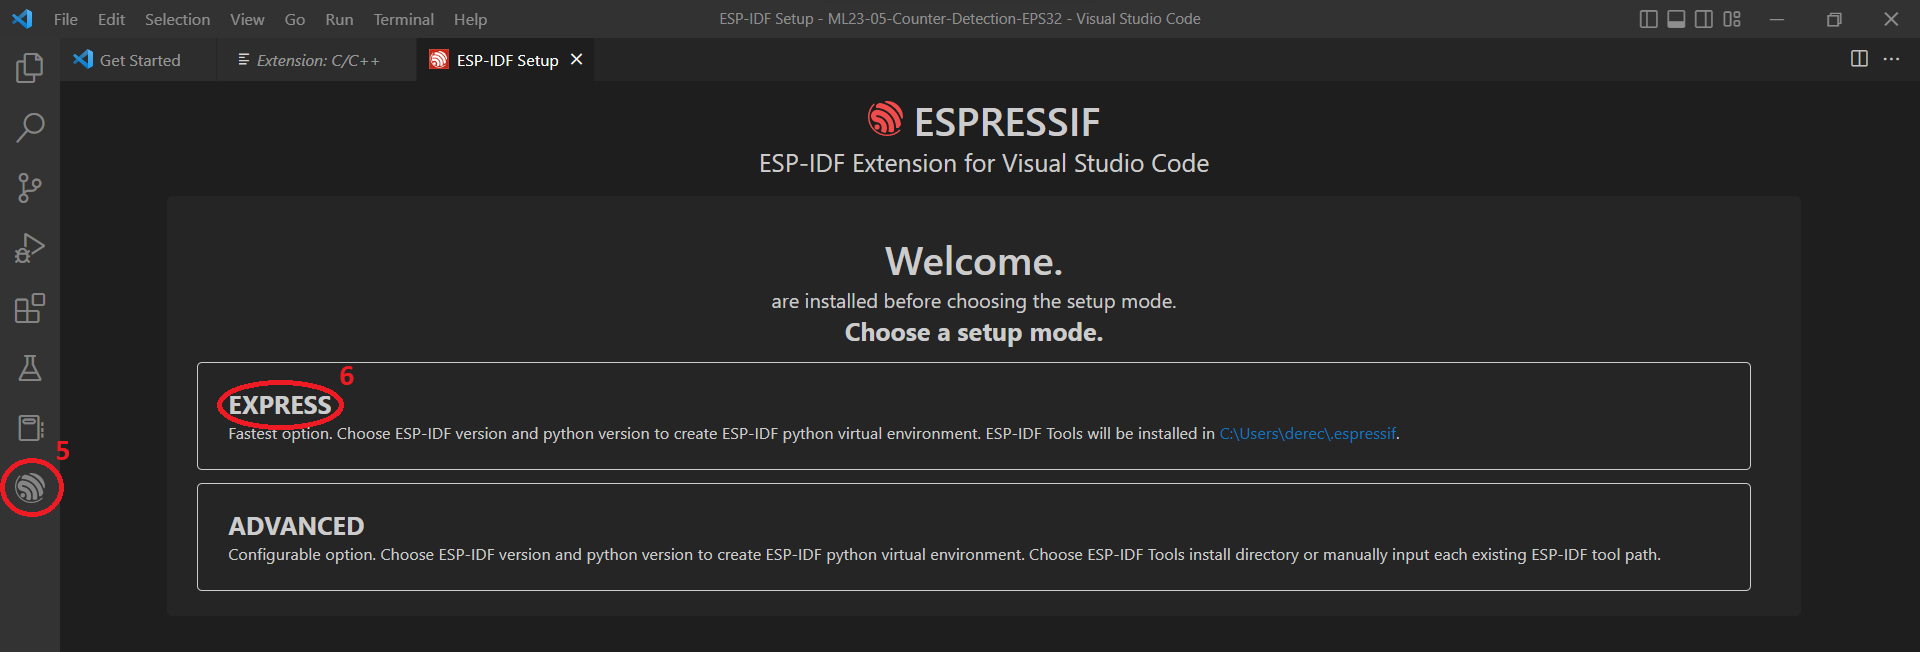
\includegraphics[width=12cm]{ESP32/ESPIDFInst2}
            \caption{Configure ESP-IDF extension: Express.} 
            \label{fig:Configure ESP-IDF extension: Express.}
        \end{center}
    \end{figure}
    \item Select Download Server: "Github".	
    \item Select an ESP-IDF version to download (v4.4.3).
    \begin{figure}  [H]
        \begin{center}
            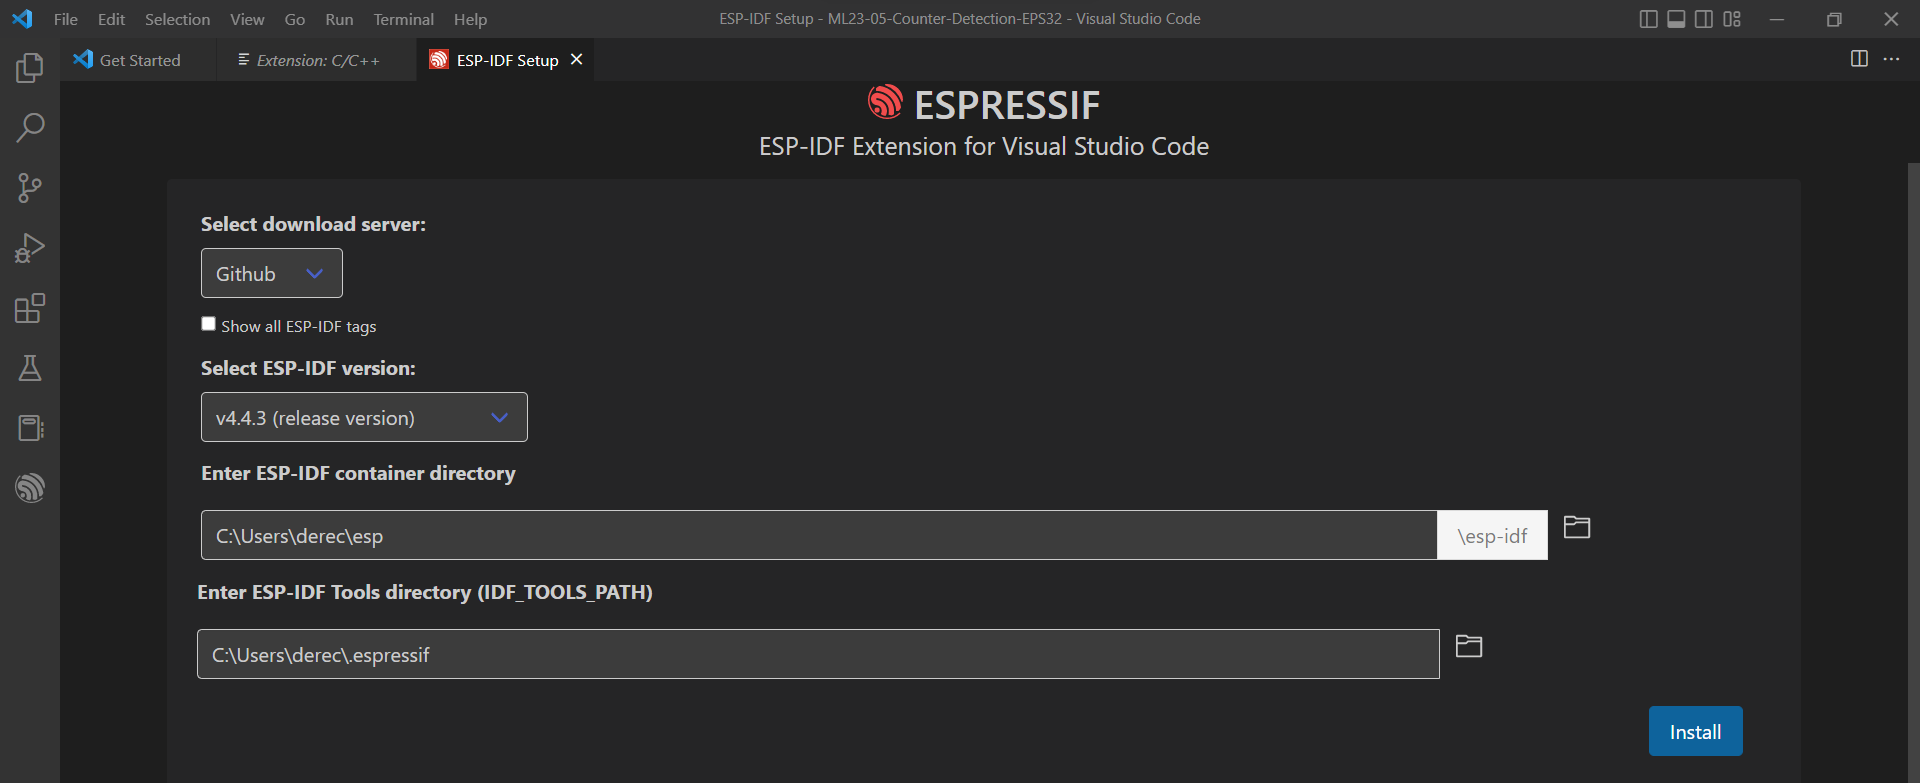
\includegraphics[width=12cm]{ESP32/ESPIDFInst3}
            \caption{Download ESP-IDF version from: GitHub.} 
            \label{fig:Download ESP-IDF version from: GitHub.}
        \end{center}
    \end{figure}	
    Once the Plug-In is properly installed in \ac{vscode}, a success message will appear in the screen. \cite{Ignacio:2022}:
    \begin{figure}  [H]
        \begin{center}
            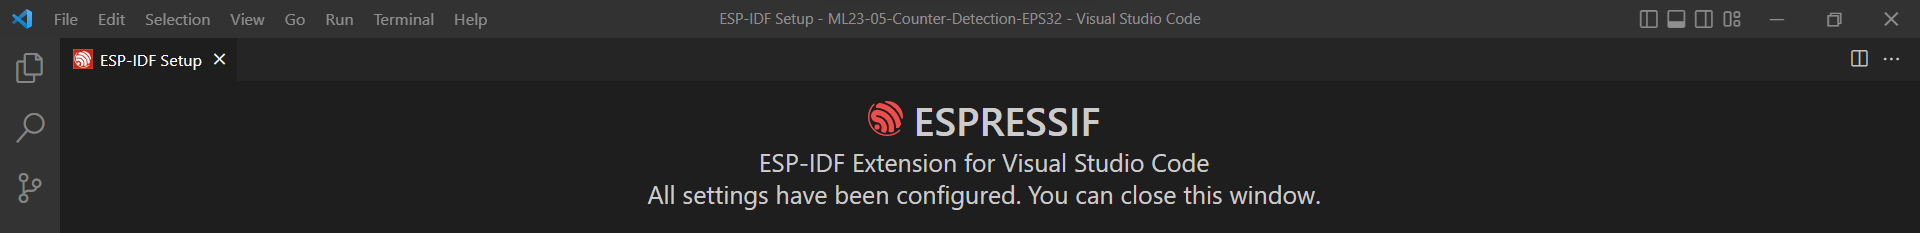
\includegraphics[width=12cm]{ESP32/ESPIDFInst4}
            \caption{Successfully installed ESP-IDF.} 
            \label{fig:Successfully installed ESP-IDF.}
        \end{center}
    \end{figure}	
    It is now time to to install the ESP32-CAM drivers. 
    
    The first thing to do is to clone or download and extract the repository [\href{https://github.com/espressif/esp32-camera}{ESP32 Camera GitHub project}] to the components folder of your ESP-IDF. To do this, continue with the following steps:
    \item In your Directory Navigator, go to the "ESP-IDF" pre-installed folder and look for the "components" folder. (i.e. "C:/Users/dereck/esp/esp-idf/components")
    \item Open Windows PowerShell.
    \item Run: git clone https://github.com/espressif/esp32-camera
    \begin{figure}  [H]
        \begin{center}
            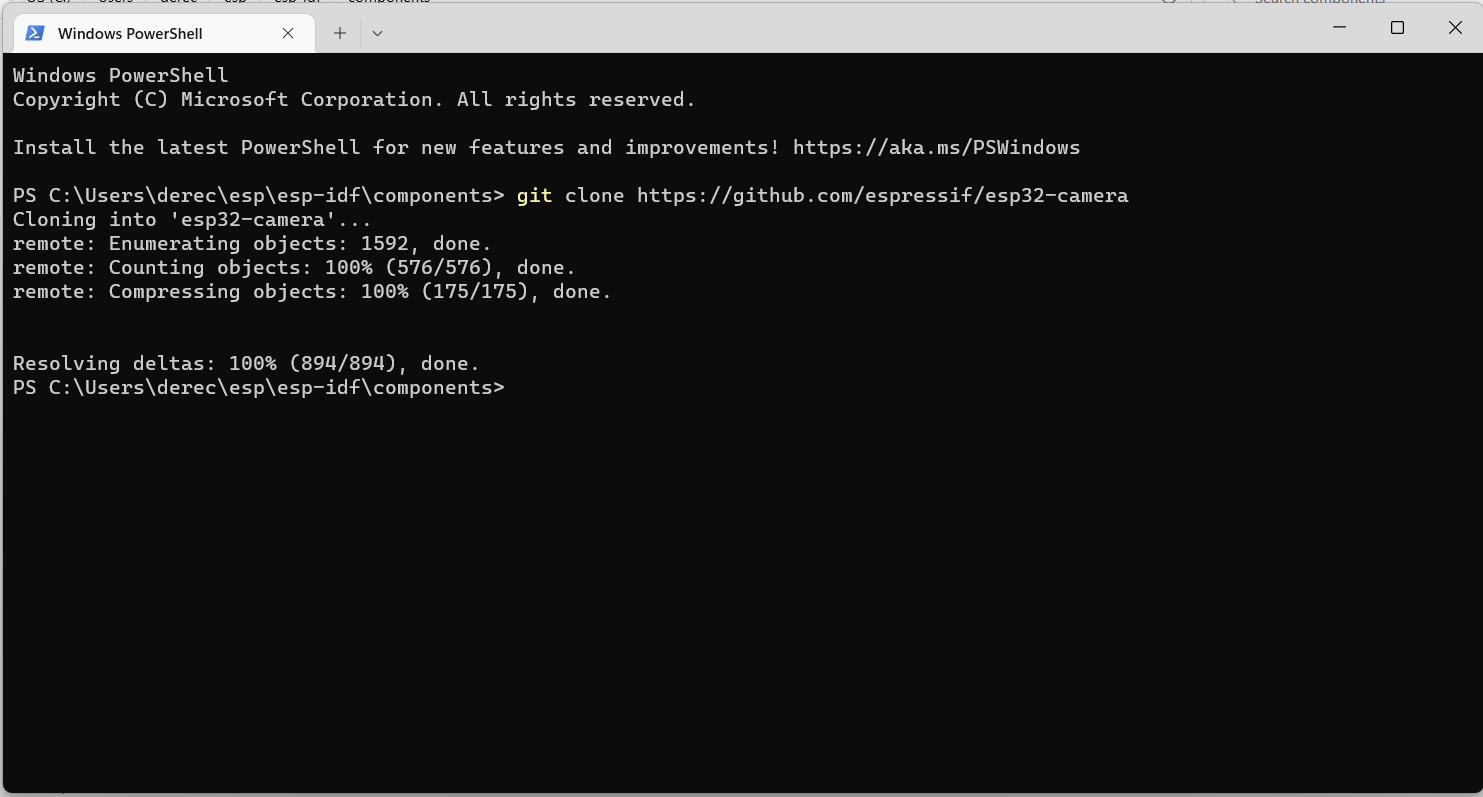
\includegraphics[width=12cm]{ESP32/ESPIDFInst5}
            \caption{ESP32 Camera Clone Repository.} 
            \label{fig:ESP32 Camera Clone Repository.}
        \end{center}
    \end{figure}	
\end{enumerate}

Now all the required drivers for the ESP32-CAM are installed and ready to be used in \ac{vscode}.

%%%%%%%%%%%%%%%%%%%%%%%%%%%%%%%

\subsection{Microprocessor Test}    
                                                            
It is now time to test basic functionalities of the microprocessor. This will be done by loading a "Hello World" function to the \ac{hw}. For this implementation the goal is to program ESP32-S microprocessor to turn on the LED integrated in the ESP32-CAM module. To achieve this, the code will upload a basic algorithm to the ESP32-CAM module. This algorithms are part of the basic test that come along with the ESP-IDF installation. Therefore the code can be found in the installation directory of this plug-in, un de this path: "examples/get-started/blink", which is relative to the installation path (i.e. C:/Users/dereck/esp/esp-idf/examples/get-started/blink).  \\

This is the code's structure:

\begin{itemize}
    \item\textbf{Include Section: }This section includes header files that are required to run specific modules on the code. These header's location have to be defined as a path in order to avoid "building errors". This definition is done under this file: ".vscode/c\_cpp\_properties.json". In particular for the this test we need the predefined path for the ESP-IDF installation (i.e. C:/Users/dereck/esp/esp-idf).
    \item\textbf{Physical Resource Definition Section: }This section is used to indicate the code what GPIO pins must interact during the code execution. In this simple case, the conde will run only on the GPIO pin dedicated for the LED on board. This GPIO pin is defined as: "define BLINK\_GPIO 33".
    \item\textbf{Functions Section: }This section includes all the sub-functions that are going to be executed during the code. In this case we have only two functions: "configure\_led", this is used to initialize the LED condition. "blink\_led", this is used to change the LED state accordingly: HIGH or LOW. 
    \item\textbf{Main Section: }This is the principal function to be executed and this section of the code will summon accordingly the pre-defined functions. 
\end{itemize}

Once the code is ready, it has to be build, meaning that \ac{vscode} will generate a project based on the original code, and "translate" this information into a machine language code to be interpreted by the ESP32-S micro controller. This is done, on the \ac{vscode} Terminal with this command: "idf.py build". \\

Finally, Once this is ready to built code needs to be flashed or loaded to the device (ESP32-CAM). In order to do this, it is used the  \ac{vscode} Terminal with this command: "idf.py -p <PORT\_NUMBER> flash monitor". <PORT\_NUMBER> is defined by the USB resource of the computer used to connect the ESP32-CAM module. \\

This is the result of the test: 

\begin{figure}  
    \begin{center}
        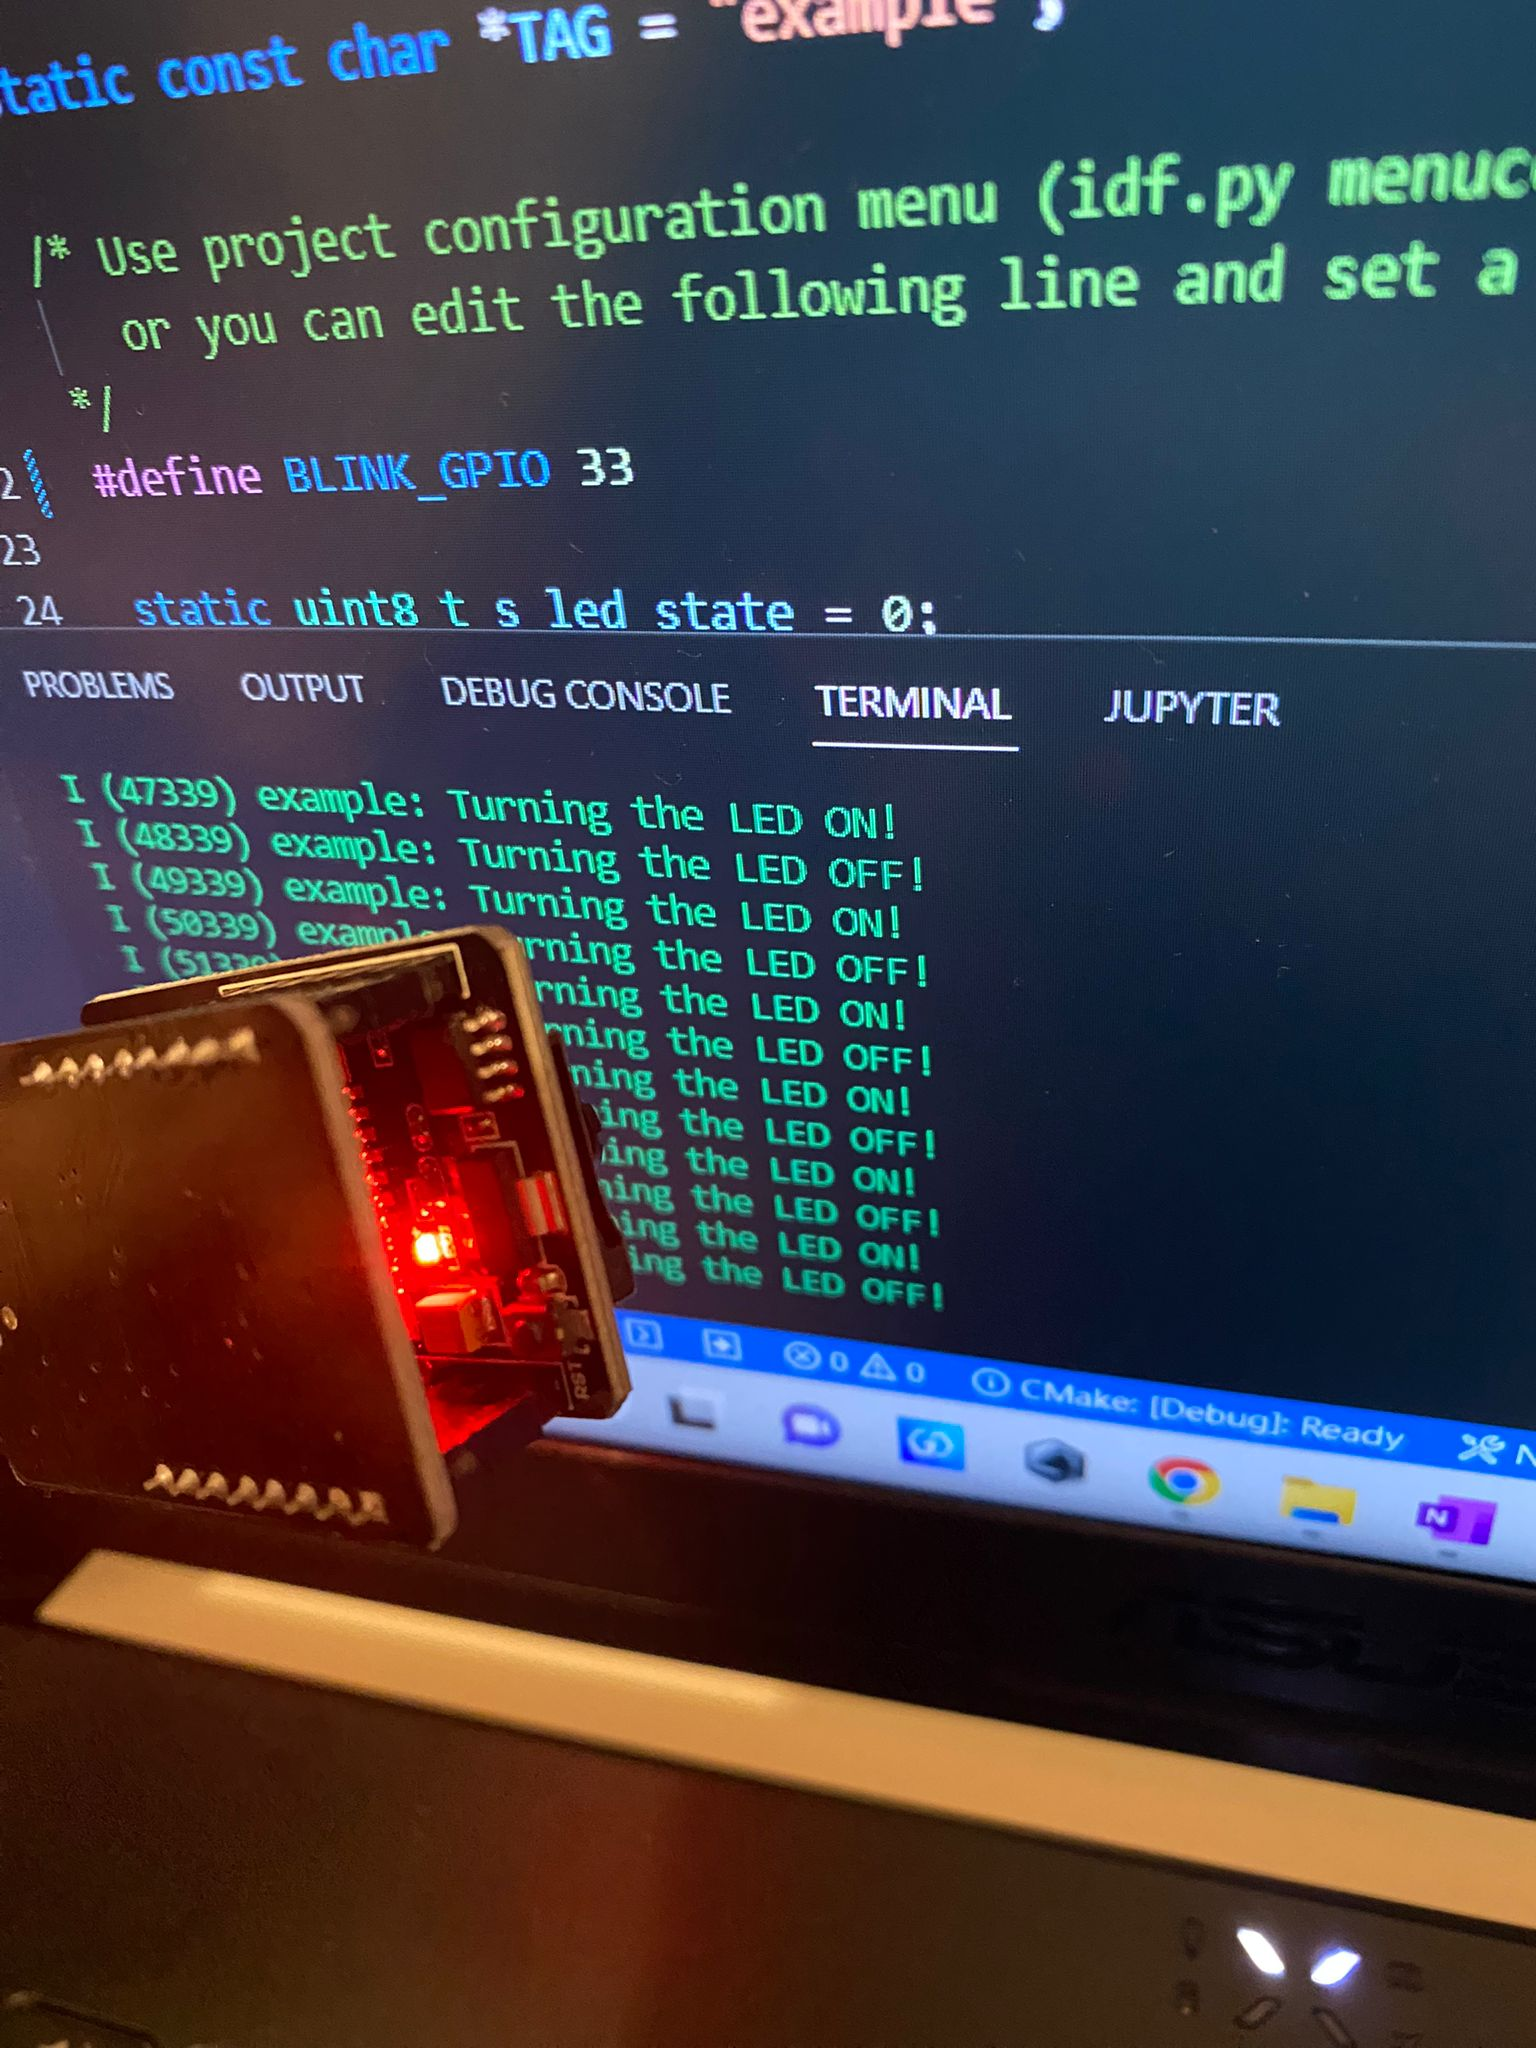
\includegraphics[width=12cm]{ESP32/ESPTest1}
        \caption{Micro processor (ESP32-S) Test in ESP32-CAM.} 
        \label{fig:Micro processor (ESP32-S) Test in ESP32-CAM.}
    \end{center}
\end{figure}	

%%%%%%%%%%%%%%%%%%%%%%%%%%%%%%%

\subsection{OV2640 Camera Test}
The other key features that are key for the project to test, before the implementation are: OV2640 Camera Interaction with ESP32-CAM, and the SD-Card, proper functionality with the module. For this end, another basic "Hello World" Function is proposed. In this case the idea is to upload a code (following somehow the same strategy as the Microprocessor Test section) in this case with four major features:
\begin{enumerate}
    \item Initialize the OV2640 Camera to take pictures.
    \item Enable the camera to take a picture every 5s.
    \item Initialize the SD-Card in the ESP32-CAM to store pictures.
    \item Store the taken pictures in the SD-Card. 
\end{enumerate}

For this example, the code will be a little more complex in order to successfully perform the required functionalities. However it will be a modular code, meaning that each function will have a separate and modular implementation, making the code easy to understand and replicate. \\

This is the code's structure:

\begin{itemize}
    \item\textbf{Include Section: }Same as previous example.
    \item\textbf{Physical Resource Definition Section: }In this case it will be targeting the "CAM\_PIN" to perform the initialization and execute the capability of capturing pictures.
    \item\textbf{Camera Basic Configuration: } This is a really important section to consider, since it was not present on the previous example. It allows the micro controller to specify the characteristic under which the camera will perfom, by setting some basic parameters.
    
    \begin{enumerate}
        \item xclk\_freq\_hz [20000000], OV2640 camera can run under 20MHz or 10MHz.
        \item pixel\_format [GRAYSCALE], can select among these options: YUV422, GRAYSCALE, RGB565 and JPEG.
        \item jpeg\_quality [12], a value between 0 and 63 to determine the picture quality (lower number means higher quality).
    \end{enumerate}

    \item\textbf{Functions Section: }For this example the utilized functions are basically to initalize the components, "init\_camera", to initialize the camera; and "init\_sdcard, to initialize the SD-Card.
    \item\textbf{Main Section: }This is the principal function to be executed, by executing this pre loaded feature: "esp\_camera\_fb\_get" to capture picture. Then assigning a name to the picture as : "picture\#". This \# is generated by a counter, that increases after each picture. 
\end{itemize}

This is the result of the test: 

\begin{figure}  
    \begin{center}
        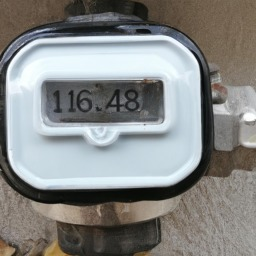
\includegraphics[width=12cm]{ESP32/ESPTest2}
        \caption{Camera (OV2640) and SD-Card Test in ESP32-CAM.} 
        \label{fig:Camera (OV2640) and SD-Card Test in ESP32-CAM.}
    \end{center}
\end{figure}	
%%%%%%%%%%%%%%%%%%%%%%%%%%%%%%%



